\documentclass[a4paper, 10pt]{scrartcl}

\usepackage[utf8]{inputenc}
\usepackage[ngerman]{babel}
\usepackage[T1]{fontenc}
\usepackage{graphicx}
\usepackage{float}
\usepackage{wrapfig}
\usepackage{fancyhdr}
\usepackage{listings}
\usepackage{color}
\usepackage{hyperref}

\definecolor{mygreen}{rgb}{0,0.6,0}
\definecolor{mygray}{rgb}{0.5,0.5,0.5}
\definecolor{mymauve}{rgb}{0.58,0,0.82}

\lstset{
basicstyle=\footnotesize, 
commentstyle=\color{mygreen},
frame=single,	
language=Java,
breaklines=true,
numbers=left,
numberstyle=\tiny\color{mygray},
showtabs=false,
tabsize=2
}

\title{Jira in der Qualitätssicherung}
\author{Charlotte Probst (Matrikel Nr. 55607)\\
 Simon Westhoff (Matrikel Nr. 56327)}
\date{03.04.2019}
\pagestyle{fancy}

\lhead{Jira in der Qualitätssicherung}
\rhead{Charlotte Probst, Simon Westhoff}
\lfoot{Semester 7}
\cfoot{\thepage}
\rfoot{Prof. Dr. rer. nat. Dirk Hoffmann}

\renewcommand{\headrulewidth}{0pt}
\renewcommand{\footrulewidth}{0pt}

\begin{document}

\maketitle

%\begin{figure}[H]
%	\centering
%	\includegraphics[width=0.5\textwidth]{Bilder/gaussian_blur.jpg}
%	\caption{Anwendung des Gauß-Filters}
%\end{figure}

\newpage

\tableofcontents

\newpage

\section{Einführung in Jira}
Jira ist eine Webanwendung die heutzutage in fast jedem agilen Projekt zum Einsatz kommt. JIRA ist eine Software zur Vorgangs- und Projektverfolgung, sie begleitet meist den gesamten Lebenszyklus eines Projekts. Sie wurde in Java programmiert und 2002 von Atlassian released. Atlassian ist ein Anbieter von Softwarelösungen für Softwareentwickler. Es hat sich im Laufe der Jahre mit mehreren namhaften Webanwendungen wie Bamboo, BitBucket und anderen Produkten für agiles Software Development zu einem unter Entwicklern sehr geschätzten Softwareunternehmen entwickelt.
\begin{itemize}
\item Jire begleitet gesamten Lebenszyklus eines Projektes oder Produktes.
\item Von der Phase der Ideensammlung über Konzeption und Umsetzung bis hin zu Fehlermanagement und Support kann Jira in jeder Phase der Wertschöpfungskette eines Unternehmens eingesetzt werden.
\item Jira bietet phasenübergreifende Konsistenz: Anforderungen, Aufgaben, Support-Tickets, Fehler etc. werden im selben System verwaltet und können dadurch miteinander in Beziehung gesetzt sowie gemeinsam durchsucht und ausgewertet werden.
\end{itemize}

\subsection{Kategorien zur Einordung unterschiedlicher Aufgaben (Vorgangstypen)}
In Jira werden verschieden Aufgabe mit Hilfe von Vorgangstypen kategorisiert. Es gibt 4 Kategorien:
\begin{enumerate}
\item \textbf{EPIC}\\
ist eine User-Story die sich über mehr als einen Sprint erstreckt.
\item \textbf{STORY}\\
besteht aus mehreren TASKs, ist eine USER-Story die sich in einem Sprint erledigen lässt ,man sollte sie in einem einfachen Satz beschreiben können.
\item \textbf{TASK}\\
entspricht einem einzelnen Aufgabenpaket.
\item \textbf{BUG}\\
ist ein Fehler, den es zu beheben gilt.
\end{enumerate}


\section{Einordnung im QS-Umfeld}
Jira ist ein sehr vielfältig einsetzbares Tool um die Zusammenarbeit unterschiedlicher Projektteilnehmer in einem agilen Softwareentwicklungsprozess zu organisieren. 
Mithilfe der SCRUM Methode kann bereits zu Beginn eines Projekts mit JIRA gearbeitet werden, durch verschiedene AddOns können unterschiedlichste Anforderungsbereiche in Projekten realisiert werden.\\
Hauptaufgaben wie die Versionierung , Bug- und Vorgangsnachverfolgerung tragen entscheidende zur Qualitätssicherung bei. Tracking, Testen und Analysieren von möglichen Fehlern werden in jede Iteration des agilen Prozesses eingebaut.
So ist eine ständige Kontrolle bzw. Dokumentation aller Arbeitsschritte für alle Projektteilnehmer möglich. \\
Testzyklen können individuelle erstellt , verwaltet und durchgeführt werden und sind dadurch auch im Nachhinein einfach nachzuverfolgen. Jira hilft also auch in der Qualitätssicherung von Code.\\
Auch Stakeholder können mit in das Projekt integriert werden und schaffen so eine höhere Zufriedenheit.

\section{Welche Funktionen bietet Jira?}

\subsection{Exkurs - Was ist Scrum?}

\textit{Erläuterung Scrum, Referenz zu Praxisbericht Charlotte Probst, SS18}\\

SCRUM beruht auf der Theorie , so wird es im  Scrumguide(Vergleich: 15.SCRUM-Guide) beschrieben , „Wissen aus Erfahrung gewonnen wird und Entscheidungen auf Basis des Bekannten getroffen werden.“ es nutzt diesen Ansatz um „Prognosesicherheit ( von Terminen und Ergebnissen) zu optimieren und Risiken zu kontrollieren“. Ein Projekt wird der aktuellen Situation und den aktuellen Problemen angepasst bzw. orientiert sich daran. 

\begin{figure}[H]
	\centering
	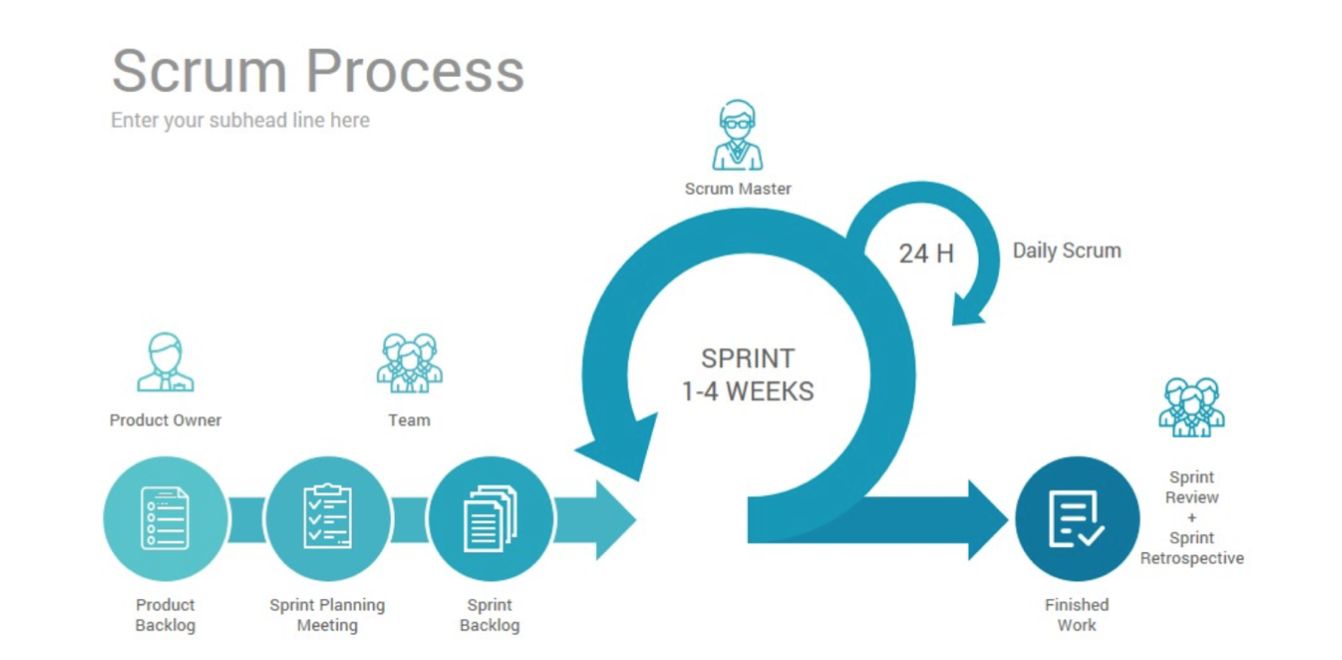
\includegraphics[width=\textwidth]{Bilder/Scrum.png}
	\caption{\url{https://brainhub.eu/blog/differences-lean-agile-scrum/}}
\end{figure}

Um diese Theorie in die Praxis erfolgreich anzuwenden beruht SCRUM auf drei Säulen : 
der Transparenz, der Überprüfung und der Anpassung.\\
Die Transparenz verhilft den Betrachtern des Projektes einen gemeinsamen Standard zu definieren. Wesentliche Aspekte des Projektes sollten für alle sichtbar sein.Man sollte seine Vorstellungen klar zusammenfassen und aufschreiben können. Zu dem sollte man für das Projekt benötigte Use Case erstellen.Das hilft den unterschiedlichen Teammitgliedern ( Produktbetreuern, Entwicklern, Managern, Stockholdern etc) sich besser im Projekte zu recht zu finden und besser mit reden bzw. Entscheidungen treffen können.\\
Die unterschiedlichen Anforderungen an das Projekt werden dann in einzelne Teile zerlegt , sodass dasTeilprojekt einen höheren Stellenwert bekommt.“Jede Version ist ein Teilsystem, die Teilsysteme bauen aufeinander auf und bilden zusammen das Gesamtsystem“(Vergleich 16 D.D. McCracken and M.A. Jackson). Diese Gesamtsystem bestehend aus seinen unabhängigen Teilsystemen kann sich dann dem jeweiligen Projekt und dessen Anforderungen besser anpassen. Benutzeranforderungen können besser integriert werden und können auch noch während des laufenden Projektes hinzugefügt werden, da man oftmals erst während den verschiedenen Teilprojekten Problematik oder andere Anforderungen erkennt. Unterschiedliche Teilprojekte und damit verbundenen Versionsmodelle haben den großen Vorteil das erste Kernsystem schon zu einem sehr frühen Zeitpunkt benutzt werden kann . Zu dem ist es möglich für das Projekt wichtige und oder kritische Aspekte in einer frühem Versionsmodell zu priorisieren.\\
Die Überprüfung erfolgt durch verschiedenste Schritte und Teammitglieder des Projekts. Projekte die mithilfe von SCRUM realisiert werden, bestehen meist aus einem Scrum-Team welches wieder rum aus einem Product Owner, einem Entwicklungsteam, dem Scrum Master und den Stakeholder zusammengesetzt ist. Je nach Projekt können aber verschiedenste Personen noch hinzukommen.\\
Das Team ist selbstorganisiert, es kann selbstständig entscheiden wie und wann Aufgaben erledigt werden. Der SCRUM-Master versucht das agile Projekt zu unterstützen , in dem er „allen Beteiligten hilft, die Scrum-Theorie, Praktiken,Regeln und Werte zu verstehen.“( Vergleich 15 Scrum-Guide). Er versucht die Zusammenarbeit aller Projektmitglieder zu organisieren und optimieren.\\
Der oder die Product Owner versucht bzw. versuchen das Ziel der Teilprojekte zu definieren und den anderen Projektmitglieder vor allem dem Entwicklungsteam verständlich zu erklären.Unterschiedliche Teilprojekte können in unterschiedlichen Projekten priorisiert oder vernachlässigt werden.\\
Das Entwicklungsteam kümmert sich um die unterschiedlichen Anforderungen die den Teilprojekten zu geordnet sind .Sie helfen bei der Projektplanung auch die Dauer, Aufwendigkeit und Realisierbarkeit einzuschätzen.\\
Die Überprüfung der einzelnen Arbeitsschritte erfolgt über unterschiedliche regelmäßige Treffen der Teammitglieder in unterschiedlichen Konstellationen.\\
Der Sprint ist das „Herz von Scrum“ ( Vergleich 15 Scrum-Guide), er findet ungefähr alle 14 Tage statt und betrifft alle Teammitglieder , innerhalb dessen ein „fertiges, nutzbares und potenziell auslieferbares Produktinkrement hergestellt wird. „(Vergleich 15 Scrum Guide).Hierbei werden Themen für die Umsetzung für die kommenden 2 Wochen festgelegt. Man kann sich individuell an die derzeitigen Bedürfnisse und Arbeitsbelastung anpassen. Auch kurzfristige Wünsche und Änderungen der Anwender können berücksichtigt werden. Zudem können wichtige Themen priorisiert werden. Während eines laufenden Sprints erfolgen keinen Änderungen im Ziel-Sprint getätigt.Der Zeitraum über den ein Sprint läuft darf nicht zu groß gewählt werden, Teilprojekte sollen im Vordergrund stehen und somit auch die immer wieder kehrende Erfolgserlebnisse für alle Projektmitglieder.
Es geht darum folgende Fragen zu beantworten:

\begin{itemize}
\item Was ist unsere nächste Teilprojekt ?
\item Was genau sind die Aufgaben/Ziele des Teilprojekts?
\item Welche Projektmitglieder werden zu welchen Aufgaben benötigt?
\item Wieviel Zeit wird das Teilprojekt von wem in Anspruch nehmen?
\end{itemize}

Der Sprint wird nach Vervollständigung von einem neuen Sprint abgelöst.
Ungefähr alle 4 Wochen findet die Produkt Backlog Planung statt, hierbei werden Themen mittelfristig im Backlog priorisiert. Er enthält alle Teilprojekte/Aufgaben die bekannt sind und dient als Orientierung für den Sprint. Der Backlog entwickelt sich im Laufe eines Projektes weiter, da immer wieder durch Feedback neue Anforderungen und Probleme hinzu gefügt werden können.Meistens werden einzelnen Einträge nur relativ groß verfasst und erst später verfeinert. Priorisierte Bachlog-Einträge werden dann detaillierter Ausgearbeitet und verfügen über mehr Klarheit - je niedriger die Priorisierung desto weniger Details enthalten die Einträge.\\
Sprint-Backlogs sind die priorisierten Einträge des Produkt Backlogs mit weiteren Informationen über Ziel-Sprints und das Projekt. Es spiegelt die Einschätzung des Entwicklungsteams für die notwendig erachtetet Arbeit für ein Teilprojekt.
Festgeschrieben werden die in den jeweiligen Meetings festgelegten Themen oftmals  mithilfe von Internetanwendung JIRA – sie ist eigens dafür konzeptioniert die SCRUM-Methode zu unterstützen.\\
Mithilfe von kurzen,täglichen Meetings, dem Daily Scrum, innerhalb der involvierten Projektmitglieder werden die Aufgaben der einzelnen Mitglieder überprüft, angepasst und aktualisiert. Zu dem wird die Planung für den kommenden Tag besprochen. Immer im Fokus steht dabei der Ziel-Spring und die Priorisierung bei der Abarbeitung der Spring Backlog Einträge. Das Daily Scrum hilft den Projektmitgliedern aktuelle Probleme zu identifizieren sowie Hinternisse zu beseitigen.Es ist ein entscheidendes Meeting zur Überprüfung und Anpassung.\\
SCRUM FRAMEWORK-Framework zum Management und zur Durchführung von Projekten in der Softwareentwicklung. Quelle:https://www.etventure.de/blog/digitallearning-2-agiles-arbeiten-mit-scrum/
Die dritte Säule in SCRUM ist die Anpassung. Sie verhilft dem Projekt sich weiter zu entwicklen, indem neue Anforderungen in die Projektplanung aufgenommen werden oder veränderte Anforderungen aktualisiert werden. SCRUM passt sich bzw. kann sich unterschiedlichen Projekten und deren unterschiedlichen Anforderungen und Projektmitgliedern anpassen.\\
Auch bei Bosch ist es immer wichtiger flexibel handeln zu können.Durch den Firefight-Modus des Werkes RTP1 kann sich das Entwicklerteam nicht jeden Tag vollständig um die Durchführung des aktuellen Projektes kümmern , zu dem befinden sich viele Mitarbeitern in unterschiedlichen Projekten und können so schnell den Überblick und damit die Fokussierung verlieren.\\
Damit ein das A2MM- Projekt ein Erfolg wird , greift man zur agilen Softwareentwicklung mit der SCRUM-Methode. SCRUM wird dabei so angepasst das es auf die individuellen Bedürfnisse der einzelnen Projektmitglieder abgestimmt werden kann.\\
Projektmitglieder werden mithilfe von wiederkehrenden Meetings in das Projekt integriert und können sowohl ihre Ideen ,Wünsche und Anforderungen mit einbringen als auch durch Informationsweitergabe,Übernahme von einzelnen Aufgaben oder Feedback das Projekt weiterentwickeln.

\section{Fazit}

\end{document}
